\documentclass[12pt]{article}
\usepackage{a4wide}
\usepackage{latexsym}
\usepackage{amssymb}
\usepackage{epic}
\usepackage{graphicx}
\usepackage[shortlabels]{enumitem}
%\pagestyle{empty}
\newcommand{\tr}{\mbox{\sf true}}
\newcommand{\fa}{\mbox{\sf false}}
\newcommand{\bimp}{\leftrightarrow}


\begin{document}

\section*{Automated Reasoning - Assignment series 1 }

\begin{center}
P.T. Jager, BSc. \\
Radboud universiteit Nijmegen\\
email: {\tt p.jager@student.ru.nl}
\end{center}

\subsection*{Problem 1: Magic factory}

Six trucks have to deliver various obscure building blocks to a special 
factory. There are five types of building blocks:
\begin{enumerate}[(a)]
	\item Nuzzles - 4 pallets - 700 kg 
	\item Skipples - 8 pallets - 1000 kg - \textit{Need to be cooled in
		one of the two cooled trucks}
	\item Crottles - 10 pallets - 1500 kg - \textit{Can not be in the same truck
		as Prittles}
	\item Dupples - 5 pallets - 100 kg - \textit{Not more than 2 pallets per
		truck}
	\item Prittles - $\geq 1$ pallets - 800 kg - \textit{Can not be in same 
		truck as Crottles}
\end{enumerate}
All trucks can cary a maximum of 8 pallets or 7800 kg (whichever is reached 
first.)
What is the maximum number of Prittles that can be delivered and how would the
pallets be divided over the 6 trucks?

For a complete description of the problem please see assignment. 

\subsubsection*{Solution:}

We generalize the solution for any $a$ Nuzzles, $b$ Skipples, $c$ Crottles, 
$d$ Dupples, $e$ Prittles and $f$ trucks.

For doing so we introduce $f*a + f*b + f*c + f*d + f*e$ variables which 
represent each possible pallet in each possible truck: 
\begin{enumerate}[(a)]
	\item $nuzzle_{tn}$ for $t=1,\ldots,f$ and $n=1,\ldots,a$
	\item $skipple_{tn}$ for $t=1,\ldots,f$ and $n=1,\ldots,b$
	\item $crottle_{tn}$ for $t=1,\ldots,f$ and $n=1,\ldots,c$
	\item $dupple_{tn}$ for $t=1,\ldots,f$ and $n=1,\ldots,d$
	\item $prittle_{tn}$ for $t=1,\ldots,f$ and $n=1,\ldots,e$
\end{enumerate}
All of these variables are either $0$ or $1$, when the $nuzzle_{tn}$ 
is $1$ for some $t,n$ then nuzzle $n$ is in truck $t$. Similar for the other 
building blocks.

\vspace{3mm}

In the following formulas we will use $blocks$ as a shorthand for ${nuzzle, 
skipple, crottle, dupple, prittle}$ and use $p_{tn}$ with $p \in blocks$
as a shorthand notation for eg. $nuzzle_{tn}$. The function $num(p)$ is assumed 
to give the number of desired pallets to move of a certain block $p$, eg.
$num(dupple) = d$. Similar, the function $weight(p)$ gives the weight of a 
certain pallet $p$.

\vspace{3mm}

For each building block the correct \emph{amount} of blocks need to be
transported. This is expressed in formula
\begin{equation} \label{eq:amount}
  \bigwedge_p^{blocks} (\sum_{t=1}^{f} \sum_{n=1}^{num(p)} p_{tn} = num(p))
\end{equation}

The combined \emph{weight} of all pallets in an truck can not exceed 7800kg. 
This is expressed in the formula
\begin{equation} \label{eq:weight}
 \bigwedge_t^f (\sum_p^{blocks} \sum_n^{num(p)} weight(p_{tn}) \leq 7800)
\end{equation}

Because all pallets have $f$ different positions they could be in (one for each
truck), it is necessary to express that each \emph{distinct} pallet (numbered 
$n$) is in exactly one truck.
\begin{equation} \label{eq:distinct}
  \bigwedge_p^{blocks} \bigwedge_n^{num(p)} (\sum_{t=1}^f p_{tn} = 1)
\end{equation}

The problem states that \emph{no 2 duples} can be in any truck. 
That is, for each truck the number of duples should be $\leq 1$. 
\begin{equation} \label{eq:valuable}
  \bigwedge_{t=1}^f (\sum_{n=1}^d dupple_{tn} \leq 1)
\end{equation}

All Skipples should be in one of two \emph{cooled} trucks. We give these trucks
numbers 1 and 2. 
\begin{equation} \label{eq:cooled}
  \sum_{t=1}^2 \sum_{n=1}^b p_{tn} = b
\end{equation}

All trucks should \emph{not contain Prittles if they contain Crottles}. That is,
if the number of Crottles in a truck is $\geq 1$ then the number of Prittles 
should be 0. If this
property holds then the reverse is also true (since containment is commutative).
When expressing this formula we use the function \emph{ite} (if-then-else) which
evaluates to its second argument when the first one evaluates to $true$ and 
evaluates to its third argument otherwise.
\begin{equation} \label{eq:explosive}
  \bigwedge_t^f ite 	(\sum_{n=1}^c crottle_{tn} \geq 1)\  
						(\sum_{n=1}^e prittle_{tn} = 0)\ 
						true 
\end{equation}

One additional needed constraint has to with the choice to represent $p_{tn}$
as a number. This constraint states that all $p_{tn}$ are either 1 or 0, that is
truck $t$ contains pallet $p$ numbered $n$ (1) or not (0).
\begin{equation} \label{eq:range}
  \bigwedge_p^{blocks} \bigwedge_{t=1}^f \bigwedge_{n=1}^{num(p)} 
	p_{tn} = 0 \vee p_{tn} = 1
\end{equation}

The total formula consists of the conjunction of all these formulas, that is:
\[ \bigwedge_p^{blocks} (\sum_{t=1}^{f} \sum_{n=1}^{num(p)} p_{tn} = num(p))
	\;\; \wedge \]
\[ \bigwedge_t^f (\sum_p^{blocks} \sum_n^{num(p)} weight(p_{tn}) \leq 7800)
	\;\; \wedge \]
\[ \bigwedge_p^{blocks} \bigwedge_n^{num(p)} (\sum_{t=1}^f p_{tn} = 1) 
	\;\; \wedge \]
\[ \bigwedge_{t=1}^f (\sum_{n=1}^d dupple_{tn} \leq 1) \;\; \wedge \]
\[ \sum_{t=1}^2 \sum_{n=1}^b p_{tn} = b \;\; \wedge \]
\[ \bigwedge_t^f ite 	(\sum_{n=1}^c crottle_{tn} \geq 1)\  
						(\sum_{n=1}^e prittle_{tn} = 0)\ 
						true 
	\;\; \wedge \]
\[ \bigwedge_p^{blocks} \bigwedge_{t=1}^f \bigwedge_{n=1}^{num(p)} 
	p_{tn} = 0 \vee p_{tn} = 1 \]

This formula is easily expressed in YICES syntax, for instance, for
$e=20$ and $a,b,c,d,f$ as defined in the assignment one can generate

{\footnotesize

{\tt ;; define all $p_{tn}$ }

{\tt (define nuzzle1\_1::int) }

{\tt (define nuzzle1\_2::int) }

$\cdots \cdots$

{\tt (define prittle6\_20::int) }

{\tt ;; constraint~\ref{eq:amount} (amount)}

{\tt (assert (= (+ nuzzle1\_1 nuzzle1\_2 $\cdots$ nuzzle6\_4) 4))}

{\tt (assert (= (+ stipple1\_1 stipple1\_2 $\cdots$ stipple6\_8) 8))}

$\cdots \cdots$

{\tt (assert (= (+ prittle1\_1 prittle1\_2 $\cdots$ prittle6\_20) 20))}

{\tt ;; constraint~\ref{eq:weight} (weight)}

{\tt (assert (<= (+ (* nuzzle1\_1 700) (* nuzzle1\_2 700) $\cdots$ 
		(* prittle1\_20 800)) 7800))}

{\tt (assert (<= (+ (* nuzzle2\_1 700) (* nuzzle2\_2 700) $\cdots$ 
		(* prittle2\_20 800)) 7800))}

$\cdots \cdots$

{\tt (assert (<= (+ (* prittle6\_1 700) (* prittle6\_2 700) $\cdots$ 
		(* prittle6\_20 800)) 7800))}
}

{\tt ;; constraint~\ref{eq:distinct} (distinct)}

{\tt (assert (= (+ nuzzle1\_1 nuzzle2\_1 $\cdots$ nuzzle6\_1) 1))}

{\tt (assert (= (+ nuzzle1\_2 nuzzle2\_2 $\cdots$ nuzzle6\_2) 1))}

$\cdots \cdots$

{\tt (assert (= (+ prittle1\_1 prittle2\_1 $\cdots$ prittle6\_1) 1))}

{\tt ;; constraint~\ref{eq:valuable} (no 2 duples per truck)}

{\tt (assert (<= (+ dupple1\_1 dupple1\_2 $\cdots$ dupple1\_6 ) 1))}

$\cdots \cdots$

{\tt (assert (<= (+ dupple6\_1 dupple6\_2 $\cdots$ dupple6\_6 ) 1))}

{\tt ;; constraint~\ref{eq:cooled} (cooled)}

{\tt (assert (= (+ stipple1\_1 stipple1\_2 $\cdots$ stipple2\_8) 8))}

{\tt ;; constraint~\ref{eq:explosive} (no Prittles if Crottles and vice-versa)}

{\tt (assert (ite 	($\geq$ (+ crottle1\_1 $\cdots$ crottle1\_10) 1) 
	 		(= (+ prittle1\_1 $\cdots$ prittle1\_20) 0) $true$))}

$\cdots \cdots$

{\tt (assert (ite 	($\geq$ (+ crottle6\_1 $\cdots$ crottle6\_10) 1) 
	 		(= (+ prittle6\_1 $\cdots$ prittle6\_20) 0) $true$))}

{\tt ;; constraint~\ref{eq:range} (all $p_{tn}$ should be 0 or 1)}

{\tt (assert( and(<= 0 nuzzle1\_1) (<= nuzzle1\_1 1)))}

{\tt (assert( and(<= 0 nuzzle1\_2) (<= nuzzle1\_2 1)))}

$\cdots \cdots$

{\tt (assert( and(<= 0 prittle6\_20) (<= prittle6\_20 1)))}

To now find what the maximum number of Prittles is we vary the number $e$. 
Through these experiments it is found that 18 is the largest number of Prittles
that can be transported within the given constraints.
Applying {\tt yices assignment1.ys} with $e=18$ yields a result almost 
instantly:

{\footnotesize

{\tt sat }

{\tt (= stipple6\_3 0)}

{\tt (= dupple4\_2 0)}

{\tt (= stipple3\_4 0)}

{\tt (= stipple4\_4 0)}

{\tt (= dupple6\_2 0)}

{\tt (= stipple1\_6 1)}

{\tt (= dupple5\_1 1)}

{\tt (= prittle6\_15 0)}

$\cdots \cdots$ }.

The following table expresses which packet is in which truck

\vspace{3mm}

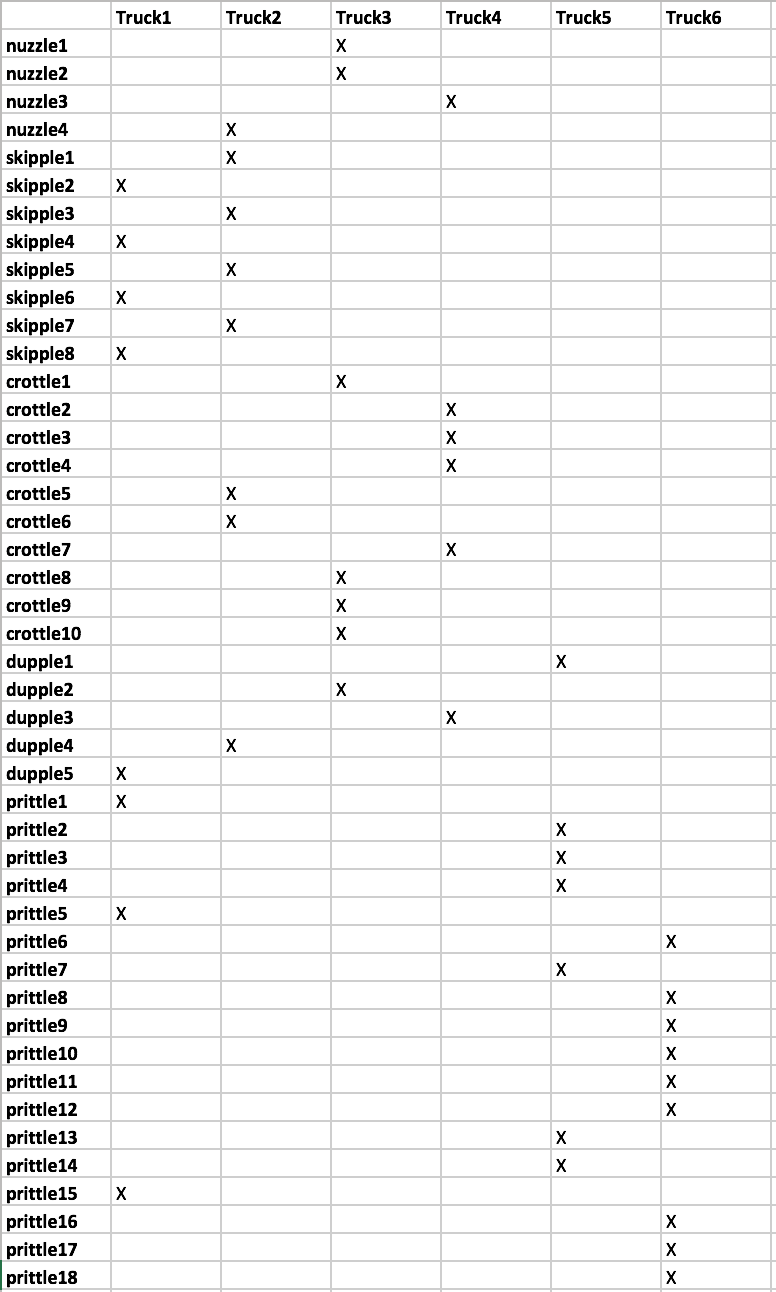
\includegraphics[angle=0]{one.png}

\end{document}
